\documentclass[graphics]{beamer}
\usepackage{xcolor}
\usepackage{graphicx}
\usepackage{verbatim}
\usepackage{wrapfig}
\usepackage{tabularx}
\usepackage{multirow}
\usepackage{amssymb}
\usepackage{pifont}
\usepackage{tikz}
\def\Checkmark{\tikz\fill[scale=0.2](0,.35) -- (.25,0) -- (1,.7) -- (.25,.15) -- cycle;} 

\useoutertheme{shadow}
%\usecolortheme{orchid}
\usecolortheme{seahorse}
\newcommand{\cmark}{\text{\ding{51}}}
%\newcommand*{\GtrSim}{\smallrel\gtrsim}

% math commands
\newcommand{\be}{\begin{eqnarray}}
\newcommand{\ee}{\end{eqnarray}}
\newcommand{\beq}{\begin{equation}}
\newcommand{\eeq}{\end{equation}}
\def\simless{\mathbin{\lower 3pt\hbox
      {$\rlap{\raise 5pt\hbox{$\char'074$}}\mathchar"7218$}}}
\def\simgreat{\mathbin{\lower 3pt\hbox
      {$\rlap{\raise 5pt\hbox{$\char'076$}}\mathchar"7218$}}} %> or of order

% variables

\def\toonscale{0.45}
\def\mboxy#1{\mbox{\small #1}}

\defbeamertemplate*{title page}{customized}[1][]
{
  \usebeamerfont{title}\inserttitle\par
  \usebeamerfont{subtitle}\usebeamercolor[fg]{subtitle}\insertsubtitle\par
  \bigskip
  \usebeamerfont{author}\insertauthor\par
  \usebeamerfont{institute}\insertinstitute\par
  \usebeamerfont{date}\insertdate\par
  \usebeamercolor[fg]{titlegraphic}\inserttitlegraphic
}
\begin{comment}
\AtBeginSection[]{
  \frame{
    \frametitle{Outline}
    \tableofcontents[currentsection]
  }
}
\end{comment}


\title{\textcolor{red}{Cosmic Lenses}}
%\subtitle{}
\author[U. Pen]{{
{ 
\textcolor{green}{\small R. Main, D. Simard, D. Baker, F. Lin,
F. Kirsten, I. Yang, V. Marthi}
}, 
\textcolor{red}{\small M. van Kerkwijk, K. Vanderlinde, JP Macquart,
  U. Pen} 
}
\\[8mm] 
}
\date{\textcolor{blue}{March 10, 2017}}


\begin{document}


%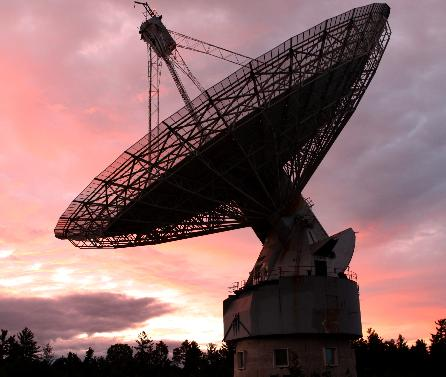
\includegraphics[width=4.4in]{Figures/IMG-7749-ARO-crop.JPG}

\frame{
\vspace{-0.5in}
\begin{center}  
%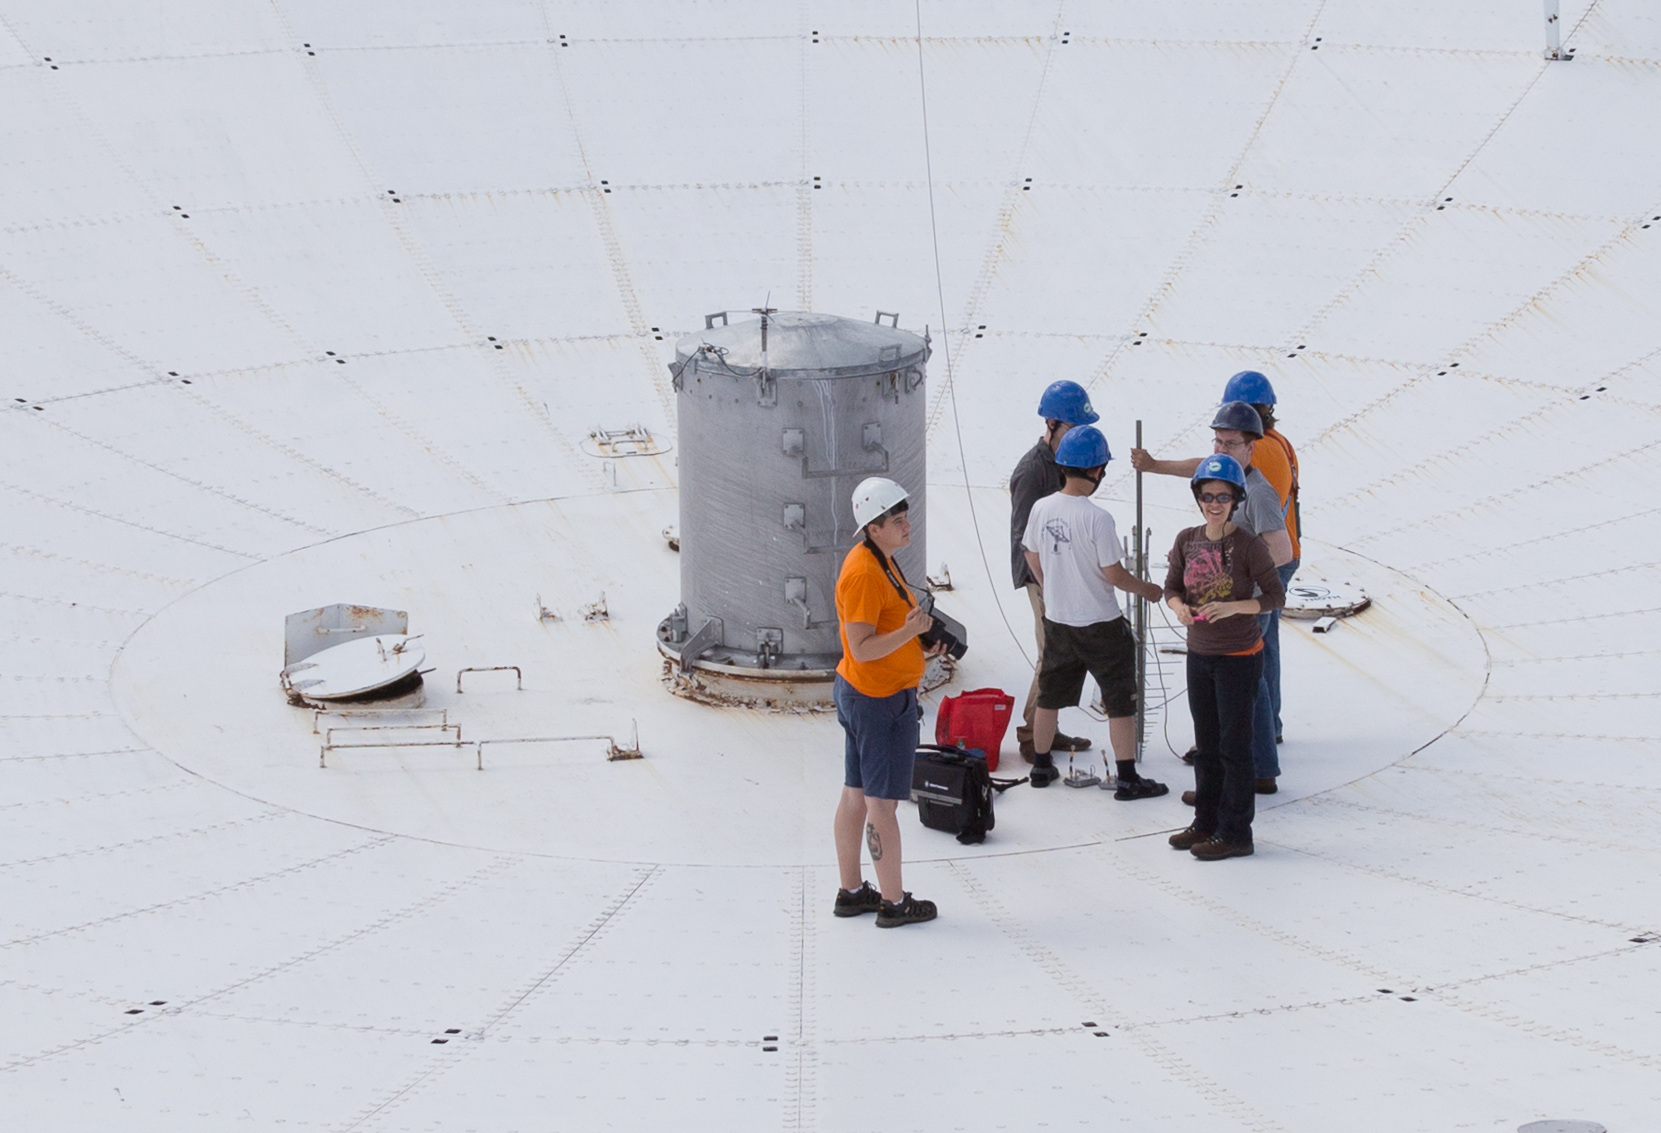
\includegraphics[width=4.4in]{Figures/IMG-0438-by-Andre-cropped.jpg}
\end{center}
\begin{picture}(320,250)
\put(-50,60){
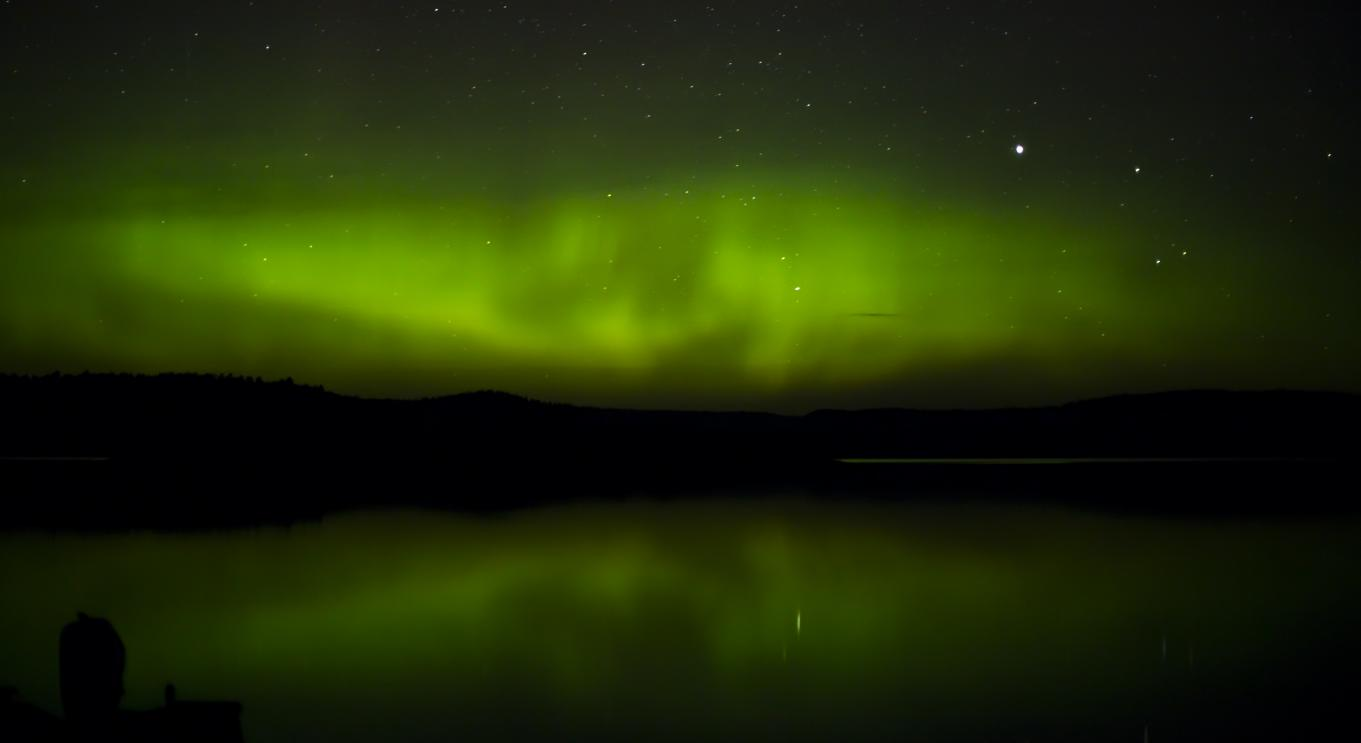
\includegraphics[width=5.5in]{Figures/traverse-aurora.jpg}}
\end{picture}
\vspace{-4in}
\\
image credit: Andre Recnik
\\
\vspace{1in}
\titlepage
}


%\section*{Introduction}
\section{Introduction}

\begin{comment}
  \subsection{Outline}

  \frame{
    \frametitle{Outline}
    \tableofcontents
  }
\end{comment}

  \frame{
    \frametitle{Overview}
    \begin{itemize}
      \item Plasma lensing: 
      \item pulsar emission, magnetospheres, FRBs
      \item ISM  magnetic fields
      \item neutron star masses, sizes, gravitational waves and more
    \end{itemize}
    \vspace{-1in}\hspace{2in}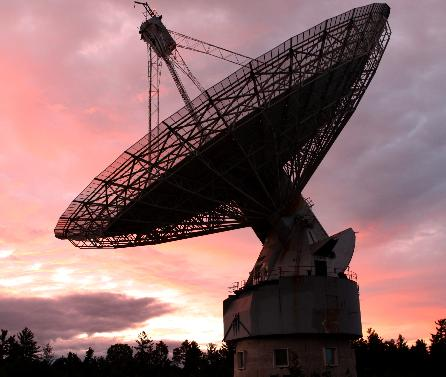
\includegraphics[width=0.5\textwidth]{Figures/IMG-7749-ARO-crop.JPG}
  }
  \frame{
    \frametitle{Scintillometry}
PSR B0834+06: 

$D_S=620$pc, 

$D_L=389/415$pc

{\tiny Brisken+2010, Liu+2016}
\begin{picture}(320,250)
\put(110,90){
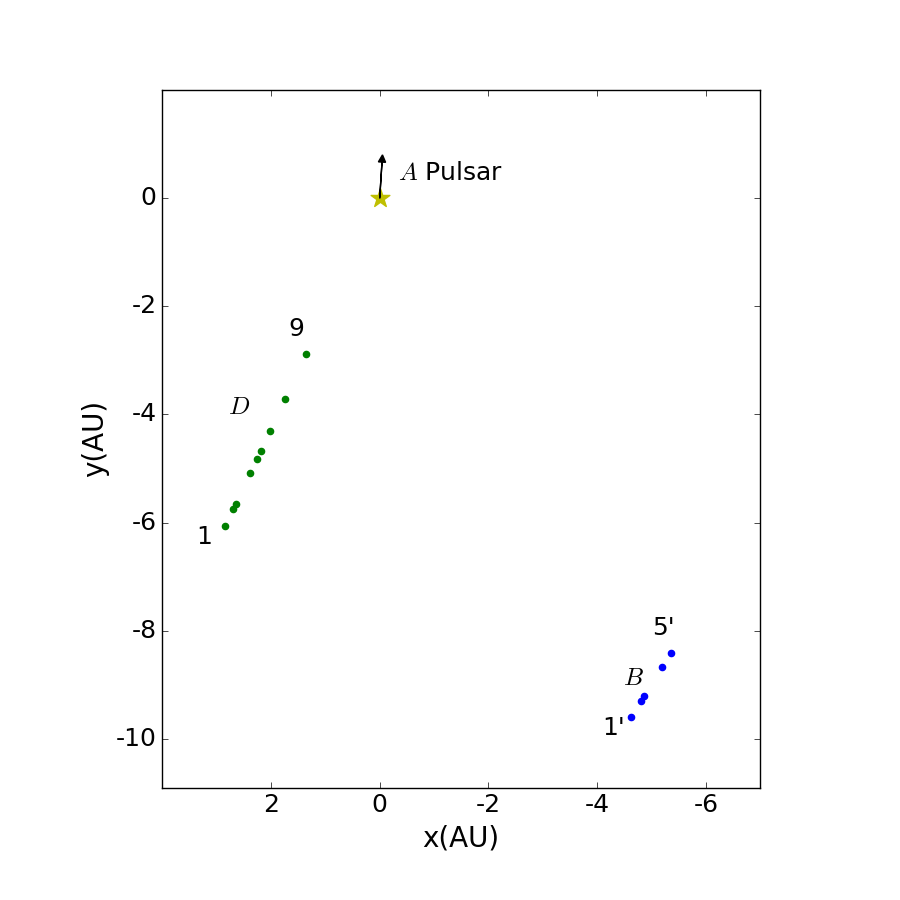
\includegraphics[width=0.7\textwidth]{Figures/Fig7_without_lines_5.png} 
}
\end{picture}
%\vspace{-4in}

  }

  \frame{
    \frametitle{Grazing incidence}
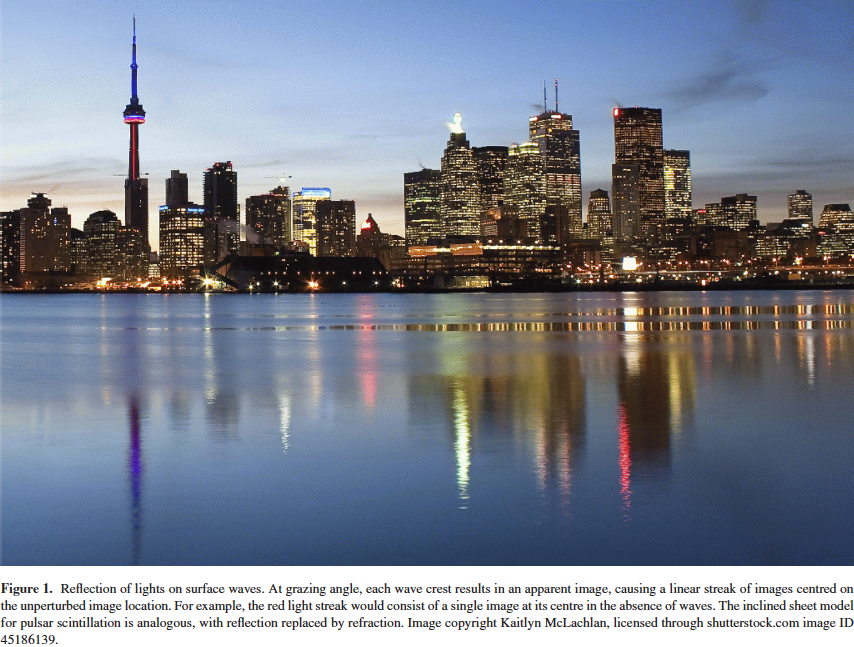
\includegraphics[width=0.9\textwidth]{Figures/toronto.png}
  }


  \frame{
    \frametitle{Lensing}
    \begin{itemize}
      \item underdense $\longrightarrow$ convergent
      \item overdense $\longrightarrow$ divergent
      \item fold $\longrightarrow$ violate odd image theorem
      \item only one image per wave period, not 4
    \end{itemize}
\vspace{-0.75in}\hspace{3.5in}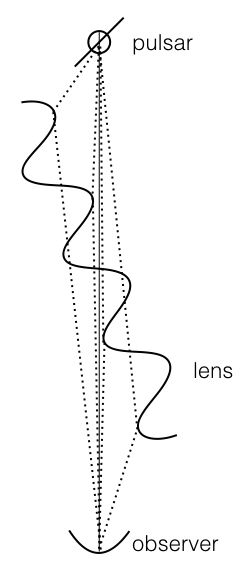
\includegraphics[width=0.25\textwidth]{Figures/convergent_geometry.jpeg}
  }
  \frame{
    \frametitle{Applications}
    \begin{itemize}
      \item cosmic telescope: picoarcsecond astrometry of magnetospheres
      \item measured 1km motion of PSR B0834+06 emission, initial results for crab
      \item potential for precision distances to pulsars, increased
        PTA sensitivity, accurate GW localization.
    \end{itemize}
%\vspace{-0.5in}\hspace{3.5in}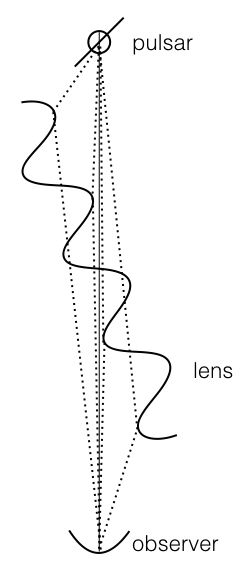
\includegraphics[width=0.15\textwidth]{Figures/convergent_geometry.jpeg}
  }
 

\end{document}
